\documentclass{article}
\usepackage{fullpage,booktabs,graphicx,hyperref,float,array}
% generated by grnbench report from result files - do not edit
\newcommand{\gbCiHighAuprcRatioAutoGrnboostTwoVsPearsonSigned}{-0.143}
\newcommand{\gbCiHighAuprcRatioAutoRegdiffusionVsPearsonSigned}{+0.126}
\newcommand{\gbCiHighAuprcRatioBaselineGrnboostTwoVsPearsonSigned}{-0.149}
\newcommand{\gbCiHighAuprcRatioBaselineRegdiffusionVsPearsonSigned}{+0.133}
\newcommand{\gbCiHighEprAutoGrnboostTwoVsPearsonSigned}{-0.471}
\newcommand{\gbCiHighEprAutoRegdiffusionVsPearsonSigned}{+0.825}
\newcommand{\gbCiHighEprBaselineGrnboostTwoVsPearsonSigned}{-0.594}
\newcommand{\gbCiHighEprBaselineRegdiffusionVsPearsonSigned}{+0.858}
\newcommand{\gbCiLowAuprcRatioAutoGrnboostTwoVsPearsonSigned}{-0.308}
\newcommand{\gbCiLowAuprcRatioAutoRegdiffusionVsPearsonSigned}{+0.010}
\newcommand{\gbCiLowAuprcRatioBaselineGrnboostTwoVsPearsonSigned}{-0.291}
\newcommand{\gbCiLowAuprcRatioBaselineRegdiffusionVsPearsonSigned}{+0.010}
\newcommand{\gbCiLowEprAutoGrnboostTwoVsPearsonSigned}{-1.134}
\newcommand{\gbCiLowEprAutoRegdiffusionVsPearsonSigned}{+0.340}
\newcommand{\gbCiLowEprBaselineGrnboostTwoVsPearsonSigned}{-1.079}
\newcommand{\gbCiLowEprBaselineRegdiffusionVsPearsonSigned}{+0.297}
\newcommand{\gbDiffAuprcRatioAutoGrnboostTwoVsPearsonSigned}{-0.225}
\newcommand{\gbDiffAuprcRatioAutoRegdiffusionVsPearsonSigned}{+0.068}
\newcommand{\gbDiffAuprcRatioBaselineGrnboostTwoVsPearsonSigned}{-0.220}
\newcommand{\gbDiffAuprcRatioBaselineRegdiffusionVsPearsonSigned}{+0.071}
\newcommand{\gbDiffEprAutoGrnboostTwoVsPearsonSigned}{-0.802}
\newcommand{\gbDiffEprAutoRegdiffusionVsPearsonSigned}{+0.582}
\newcommand{\gbDiffEprBaselineGrnboostTwoVsPearsonSigned}{-0.836}
\newcommand{\gbDiffEprBaselineRegdiffusionVsPearsonSigned}{+0.577}
\newcommand{\gbFamilyAuprcRatioAuto}{4}
\newcommand{\gbFamilyAuprcRatioBaseline}{4}
\newcommand{\gbFamilyEprAuto}{4}
\newcommand{\gbFamilyEprBaseline}{4}
\newcommand{\gbMeanAuprcRatioAutoClr}{1.302}
\newcommand{\gbMeanAuprcRatioAutoGrnboostTwo}{1.101}
\newcommand{\gbMeanAuprcRatioAutoPearsonSigned}{1.326}
\newcommand{\gbMeanAuprcRatioAutoRegdiffusion}{1.395}
\newcommand{\gbNAuprcRatioAutoGrnboostTwoVsPearsonSigned}{24}
\newcommand{\gbNAuprcRatioAutoRegdiffusionVsPearsonSigned}{24}
\newcommand{\gbNAuprcRatioBaselineGrnboostTwoVsPearsonSigned}{23}
\newcommand{\gbNAuprcRatioBaselineRegdiffusionVsPearsonSigned}{23}
\newcommand{\gbNAutoClr}{24}
\newcommand{\gbNAutoGrnboostTwo}{24}
\newcommand{\gbNAutoPearsonSigned}{24}
\newcommand{\gbNAutoRegdiffusion}{24}
\newcommand{\gbNDatasets}{40}
\newcommand{\gbNEprAutoGrnboostTwoVsPearsonSigned}{24}
\newcommand{\gbNEprAutoRegdiffusionVsPearsonSigned}{24}
\newcommand{\gbNEprBaselineGrnboostTwoVsPearsonSigned}{23}
\newcommand{\gbNEprBaselineRegdiffusionVsPearsonSigned}{23}
\newcommand{\gbPHolmAuprcRatioAutoGrnboostTwoVsPearsonSigned}{1.000}
\newcommand{\gbPHolmAuprcRatioAutoRegdiffusionVsPearsonSigned}{0.036}
\newcommand{\gbPHolmAuprcRatioBaselineGrnboostTwoVsPearsonSigned}{1.000}
\newcommand{\gbPHolmAuprcRatioBaselineRegdiffusionVsPearsonSigned}{0.038}
\newcommand{\gbPHolmEprAutoGrnboostTwoVsPearsonSigned}{1.000}
\newcommand{\gbPHolmEprAutoRegdiffusionVsPearsonSigned}{9.3e-05}
\newcommand{\gbPHolmEprBaselineGrnboostTwoVsPearsonSigned}{1.000}
\newcommand{\gbPHolmEprBaselineRegdiffusionVsPearsonSigned}{0.00047}
\newcommand{\gbPHolmRevAuprcRatioAutoGrnboostTwoVsPearsonSigned}{1.9e-05}
\newcommand{\gbPHolmRevAuprcRatioAutoRegdiffusionVsPearsonSigned}{1.000}
\newcommand{\gbPHolmRevAuprcRatioBaselineGrnboostTwoVsPearsonSigned}{3.5e-06}
\newcommand{\gbPHolmRevAuprcRatioBaselineRegdiffusionVsPearsonSigned}{1.000}
\newcommand{\gbPHolmRevEprAutoGrnboostTwoVsPearsonSigned}{9.3e-05}
\newcommand{\gbPHolmRevEprAutoRegdiffusionVsPearsonSigned}{1.000}
\newcommand{\gbPHolmRevEprBaselineGrnboostTwoVsPearsonSigned}{7.2e-07}
\newcommand{\gbPHolmRevEprBaselineRegdiffusionVsPearsonSigned}{1.000}

\title{EXP-20261001-LD-1: Exploratory contextual stress and complete real-data validation}
\author{grnbench report generated from EXP-20261001-LD-1}
\date{}
\begin{document}
\maketitle
\section*{Status}
Experiment EXP-20261001-LD-1, type: exploratory. Record status: done. Both phases are completely accounted for; this remains exploratory and does not support a headline or confirmatory claim. Reproduced by: pending; exploratory results do not enter paper/.
\section{Configuration summary}
\begin{table}[H]\centering\small
\caption{Configuration of the run, from the experiment record and the run folder.}
\begin{tabular}{p{0.3\linewidth}p{0.62\linewidth}}\toprule
experiment & EXP-20261001-LD-1 \\
type & exploratory. This run validates new simulator/runner machinery and estimates stress curves; it cannot support a headline or paper claim without a separately registered confirmatory rerun \\
owner & LD (agent-run)   issue: \#23   registered: 2026-10-01 \\
datasets (rows) & 40 \\
models & clr, grnboost2, pearson\_signed, regdiffusion \\
arms & auto, baseline \\
code & clean commit on branch ld/contextual-stress-bench; hpc/hpc.sh sync writes its hash to GIT\_COMMIT, and each job copies that into CODE\_COMMIT. The task SHA256 and score-affecting options are pinned separately in tasks.json and RUN\_CONFIG.json. \\
code commit (run folder) & 9743907d659510c4b63d53473adae7cc7bfc79b0 \\
environment & Bocconi HPC conda env grnbench, Python 3.11, requirements/lock-py311.txt plus its pinned RegDiffusion/CPU-torch header line via WITH\_TORCH=1 bash hpc/setup\_env.sh. \\
machine & Bocconi HPC, partition/QOS stud, one job at a time, 8 CPUs, 32 GB, 24 h. Work files use \textasciitilde{}/gb\_tmp, not compute-node /tmp; resubmission uses the identical command and output folder. \\
seeds & scenario seeds 0-4; union-truth split seed = scenario seed; score-cell subsample seed 0; GRNBoost2 seed 42; RegDiffusion seed 0. Shared edges are split before context expansion, so the same shared edge can never enter selection for one type and evaluation for another. \\
run folder & benchmarks/results/EXP-20261001-LD-1/real \\
generated & 2026-10-02 14:31 \\
\bottomrule\end{tabular}\end{table}

\section{Methods}
\begin{description}
\item[type] exploratory. This run validates new simulator/runner machinery and estimates stress curves; it cannot support a headline or paper claim without a separately registered confirmatory rerun
\item[question] does the context-specific simulator and status-aware benchmark complete every planned synthetic and approved real-data task without silent omissions, and at what declared severity does each model first lose recovery or operability?
\item[seeds] scenario seeds 0-4; union-truth split seed = scenario seed; score-cell subsample seed 0; GRNBoost2 seed 42; RegDiffusion seed 0. Shared edges are split before context expansion, so the same shared edge can never enter selection for one type and evaluation for another.
\item[models] pearson\_signed, clr, grnboost2, regdiffusion. Expensive models are evaluated only on distinct baseline/rules/auto candidates and never select a pipeline on the evaluation truth. Exploratory compute parameters: GRNBoost2 n\_estimators=100; RegDiffusion n\_steps=100, CPU. Motif models are excluded so unresolved issue \#21 does not add a second reference-like input.
\item[code] clean commit on branch ld/contextual-stress-bench; hpc/hpc.sh sync writes its hash to GIT\_COMMIT, and each job copies that into CODE\_COMMIT. The task SHA256 and score-affecting options are pinned separately in tasks.json and RUN\_CONFIG.json.
\item[environment] Bocconi HPC conda env grnbench, Python 3.11, requirements/lock-py311.txt plus its pinned RegDiffusion/CPU-torch header line via WITH\_TORCH=1 bash hpc/setup\_env.sh.
\item[machine] Bocconi HPC, partition/QOS stud, one job at a time, 8 CPUs, 32 GB, 24 h. Work files use \textasciitilde{}/gb\_tmp, not compute-node /tmp; resubmission uses the identical command and output folder.
\item[models scored] clr, grnboost2, pearson\_signed, regdiffusion
\end{description}

\section{Results}
\subsection{Primary comparison}
No machine-readable primary comparison in the record (field \texttt{primary comparison: A > B | metric | arm}); results are descriptive.

\subsection{Performance per model, across datasets}
\begin{table}[H]\centering\small
\caption{Reference recovery per model (CollecTRI evaluation half; AUPRC ratio, 1 = random). Unit = dataset; n per model shown.}
\begin{tabular}{lrrrr}\toprule
model & n & mean (auto) & median (auto) & mean (baseline) \\ \midrule
regdiffusion & 24 & 1.395 & 1.350 & 1.395 \\
pearson\_signed & 24 & 1.326 & 1.278 & 1.324 \\
clr & 24 & 1.302 & 1.305 & 1.317 \\
grnboost2 & 24 & 1.101 & 1.100 & 1.104 \\
\bottomrule\end{tabular}\end{table}

\subsection{Performance per dataset}
\begin{table}[H]\centering\scriptsize
\caption{AUPRC ratio per dataset, auto pipeline (1 = random); the unit of analysis.}
\resizebox{\linewidth}{!}{\begin{tabular}{lrrrr}\toprule
dataset & regdiffusion & pearson\_signed & clr & grnboost2 \\ \midrule
beeline\_\_GSD-2000-1 & n/a & n/a & n/a & n/a \\
beeline\_\_GSD-2000-10 & n/a & n/a & n/a & n/a \\
beeline\_\_GSD-2000-2 & n/a & n/a & n/a & n/a \\
beeline\_\_GSD-2000-3 & n/a & n/a & n/a & n/a \\
beeline\_\_GSD-2000-4 & n/a & n/a & n/a & n/a \\
beeline\_\_GSD-2000-5 & n/a & n/a & n/a & n/a \\
beeline\_\_GSD-2000-6 & n/a & n/a & n/a & n/a \\
10x-3-v2\_\_homo-sapiens\_\_entorhinal-cortex\_\_9f104 & 1.21 & 1.21 & 1.13 & 1.04 \\
10x-3-v2\_\_homo-sapiens\_\_superior-frontal-gyrus\_\_ & 1.35 & 1.39 & 1.17 & 1.07 \\
10x-3-v2\_\_microcebus-murinus\_\_hypothalamus-pitui & n/a & n/a & n/a & n/a \\
10x-3-v2\_\_microcebus-murinus\_\_uterus\_\_f69adac8 & n/a & n/a & n/a & n/a \\
10x-3-v2\_\_mus-musculus\_\_large-intestine\_\_de4e7a0 & 1.54 & 1.26 & 1.37 & 1.13 \\
10x-3-v2\_\_mus-musculus\_\_spinal-cord\_\_989a76f9 & 1.15 & 1.25 & 1.12 & 1.07 \\
10x-3-v3\_\_callithrix-jacchus\_\_hippocampal-format & n/a & n/a & n/a & n/a \\
10x-3-v3\_\_callithrix-jacchus\_\_primary-motor-cort & n/a & n/a & n/a & n/a \\
10x-3-v3\_\_homo-sapiens\_\_liver\_\_d7476ae2 & 1.94 & 2.00 & 1.62 & 1.08 \\
10x-3-v3\_\_homo-sapiens\_\_prostate-gland\_\_182f8181 & 1.32 & 1.18 & 1.36 & 1.08 \\
10x-3-v3\_\_macaca-mulatta\_\_primary-motor-cortex\_\_ & n/a & n/a & n/a & n/a \\
10x-3-v3\_\_mus-musculus\_\_cervical-spinal-cord\_\_9f & 1.20 & 0.97 & 1.23 & 1.10 \\
10x-3-v3\_\_mus-musculus\_\_diencephalon\_\_6de332e1 & 1.16 & 1.21 & 1.20 & 1.15 \\
10x-5-v1\_\_homo-sapiens\_\_lung\_\_703f00e6 & 1.65 & 1.30 & 1.45 & 1.11 \\
10x-5-v1\_\_homo-sapiens\_\_lung\_\_cdefb878 & 1.40 & 1.23 & 1.33 & 1.15 \\
10x-5-v2\_\_homo-sapiens\_\_blood\_\_ee782eb7 & 1.66 & 1.66 & 1.68 & 1.13 \\
10x-5-v2\_\_mus-musculus\_\_caecum\_\_0a1ad9d5 & 1.30 & 1.30 & 1.26 & 1.13 \\
10x-5-v2\_\_mus-musculus\_\_caecum\_\_95dfddd0 & 1.35 & 1.36 & 1.27 & 1.16 \\
10x-gene-expression-flex\_\_homo-sapiens\_\_blood\_\_9 & 1.50 & 1.47 & 1.31 & 1.11 \\
10x-multiome\_\_homo-sapiens\_\_atrioventricular-nod & 1.47 & 1.25 & 1.30 & 1.07 \\
bd-rhapsody-targeted-mrna\_\_homo-sapiens\_\_blood\_\_ & 1.21 & 1.37 & 1.10 & 1.17 \\
cel-seq2\_\_homo-sapiens\_\_left-main-bronchus\_\_03da & 1.40 & 1.40 & 1.26 & 1.10 \\
cel-seq\_\_homo-sapiens\_\_epithelium-of-main-bronch & 1.35 & 1.16 & 1.32 & 1.05 \\
modified-strt-seq\_\_homo-sapiens\_\_interventricula & 1.34 & 1.32 & 1.26 & 1.04 \\
patch-seq\_\_mus-musculus\_\_primary-motor-cortex\_\_8 & 1.31 & 1.22 & 1.14 & 1.13 \\
sci-rna-seq3\_\_danio-rerio\_\_endocrine-pancreas\_\_e & n/a & n/a & n/a & n/a \\
sci-rna-seq3\_\_macaca-mulatta\_\_brodmann-1909-area & n/a & n/a & n/a & n/a \\
sci-rna-seq3\_\_mus-musculus\_\_embryo\_\_0bcda669 & 1.31 & 1.24 & 1.31 & 1.06 \\
smart-seq2\_\_homo-sapiens\_\_islet-of-langerhans\_\_6 & 1.27 & 1.21 & 1.31 & 1.06 \\
smart-seq2\_\_mus-musculus\_\_aorta\_\_0380ddce & 1.45 & 1.55 & 1.37 & 1.20 \\
paul15 & n/a & n/a & n/a & n/a \\
pbmc3k\_filtered & 1.60 & 1.31 & 1.36 & 1.07 \\
pbmc3k\_raw & n/a & n/a & n/a & n/a \\
\midrule
mean & 1.39 & 1.33 & 1.30 & 1.10 \\
median & 1.35 & 1.28 & 1.31 & 1.10 \\
SD & 0.19 & 0.20 & 0.14 & 0.04 \\
\bottomrule\end{tabular}}\end{table}

\subsection{Comparative summary: declared comparisons}
\begin{table}[H]\centering\small
\caption{Declared comparisons, AUPRC ratio, auto pipeline: paired t over datasets (compare\_units), two-sided per direction, Holm over 4 directed hypotheses; 95\% interval of the mean paired difference.}
\begin{tabular}{llrrlrrl}\toprule
A & B & n & mean A$-$B & 95\% interval & $p_{A>B}$ Holm & $p_{B>A}$ Holm & supported \\ \midrule
grnboost2 & pearson\_signed & 24 & -0.225 & [-0.308, -0.143] & 1.000 & 1.9e-05 & pearson\_signed \\
regdiffusion & pearson\_signed & 24 & +0.068 & [+0.010, +0.126] & 0.036 & 1.000 & regdiffusion \\
\bottomrule\end{tabular}\end{table}

\begin{table}[H]\centering\small
\caption{Declared comparisons, AUPRC ratio, baseline pipeline: paired t over datasets (compare\_units), two-sided per direction, Holm over 4 directed hypotheses; 95\% interval of the mean paired difference.}
\begin{tabular}{llrrlrrl}\toprule
A & B & n & mean A$-$B & 95\% interval & $p_{A>B}$ Holm & $p_{B>A}$ Holm & supported \\ \midrule
grnboost2 & pearson\_signed & 23 & -0.220 & [-0.291, -0.149] & 1.000 & 3.5e-06 & pearson\_signed \\
regdiffusion & pearson\_signed & 23 & +0.071 & [+0.010, +0.133] & 0.038 & 1.000 & regdiffusion \\
\bottomrule\end{tabular}\end{table}

\begin{table}[H]\centering\small
\caption{Declared comparisons, EPR, auto pipeline: paired t over datasets (compare\_units), two-sided per direction, Holm over 4 directed hypotheses; 95\% interval of the mean paired difference.}
\begin{tabular}{llrrlrrl}\toprule
A & B & n & mean A$-$B & 95\% interval & $p_{A>B}$ Holm & $p_{B>A}$ Holm & supported \\ \midrule
grnboost2 & pearson\_signed & 24 & -0.802 & [-1.134, -0.471] & 1.000 & 9.3e-05 & pearson\_signed \\
regdiffusion & pearson\_signed & 24 & +0.582 & [+0.340, +0.825] & 9.3e-05 & 1.000 & regdiffusion \\
\bottomrule\end{tabular}\end{table}

\begin{table}[H]\centering\small
\caption{Declared comparisons, EPR, baseline pipeline: paired t over datasets (compare\_units), two-sided per direction, Holm over 4 directed hypotheses; 95\% interval of the mean paired difference.}
\begin{tabular}{llrrlrrl}\toprule
A & B & n & mean A$-$B & 95\% interval & $p_{A>B}$ Holm & $p_{B>A}$ Holm & supported \\ \midrule
grnboost2 & pearson\_signed & 23 & -0.836 & [-1.079, -0.594] & 1.000 & 7.2e-07 & pearson\_signed \\
regdiffusion & pearson\_signed & 23 & +0.577 & [+0.297, +0.858] & 0.00047 & 1.000 & regdiffusion \\
\bottomrule\end{tabular}\end{table}

\section{Visualizations and explainability}
\begin{figure}[H]\centering
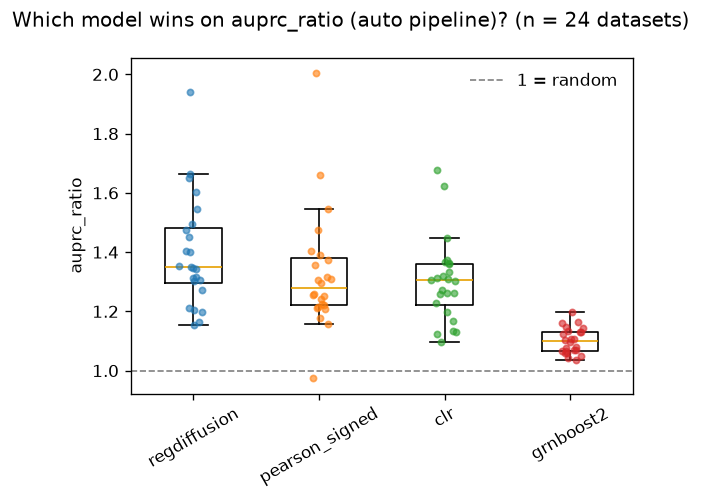
\includegraphics[width=0.85\linewidth]{../viz/scores_auprc_ratio_auto.png}
\caption{-   (n = 24 datasets) - built from  rows/ .json (auto/auprc\_ratio)}
\end{figure}
\begin{figure}[H]\centering
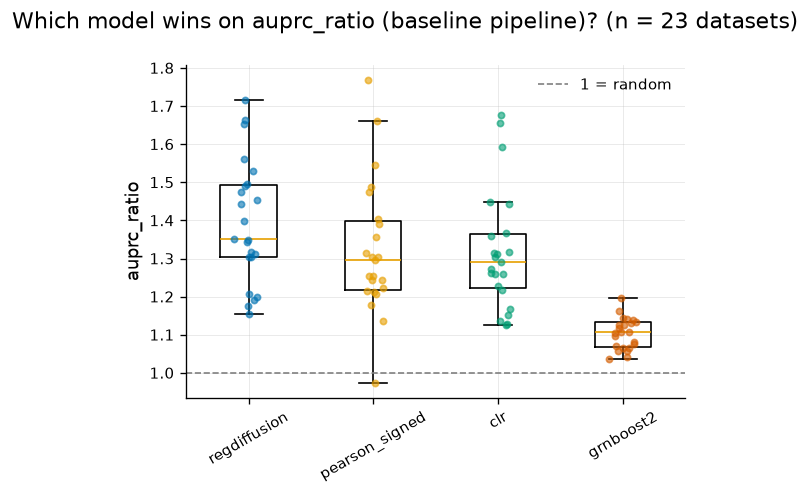
\includegraphics[width=0.85\linewidth]{../viz/scores_auprc_ratio_baseline.png}
\caption{-   (n = 23 datasets) - built from  rows/ .json (baseline/auprc\_ratio)}
\end{figure}
\begin{figure}[H]\centering
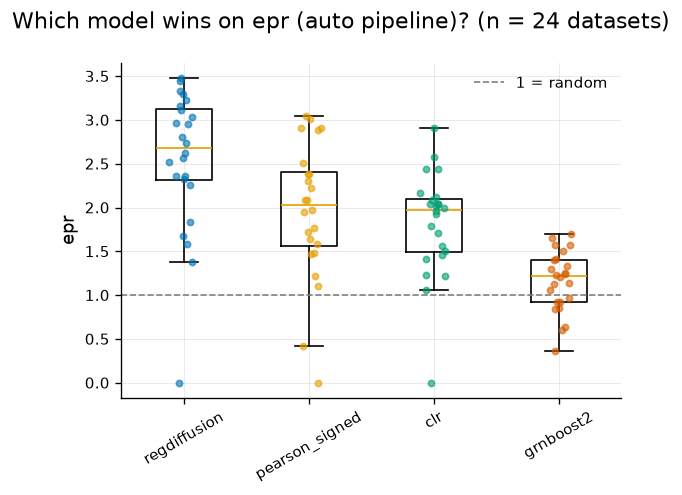
\includegraphics[width=0.85\linewidth]{../viz/scores_epr_auto.png}
\caption{-   (n = 24 datasets) - built from  rows/ .json (auto/epr)}
\end{figure}
\begin{figure}[H]\centering
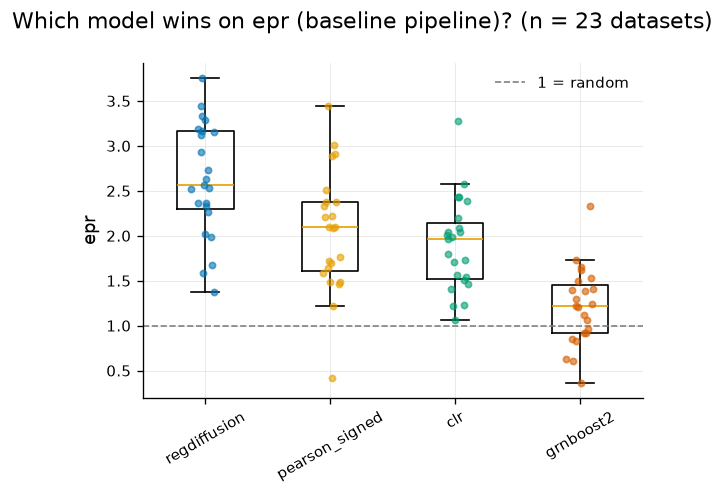
\includegraphics[width=0.85\linewidth]{../viz/scores_epr_baseline.png}
\caption{-   (n = 23 datasets) - built from  rows/ .json (baseline/epr)}
\end{figure}

\section{Limitations}
\begin{itemize}
\item Exploratory experiment: results need a confirmatory rerun before a headline claim.
\item Recorded deviation: on 2026-10-02 the completed rows exposed analysis-only report defects. The visualization reader did not understand the D-019 manifest wrapper, missing decisions became pandas NaN, and scoreless completed rows were labelled "ok, scored". Fixes and regression tests were committed, then reports were regenerated from the unchanged rows; models were not rerun. Synthetic stress figures and a generated global-only portable real overview were added from the unchanged result tables. The executed task manifest also contained an HPC home path, so it stays off git; a generated portable manifest replaces the home prefix with \textasciitilde{}/ and preserves the executed source hash. These changes affect reporting and portability only, not scores.
\end{itemize}

\end{document}
